\appendix
\chapter{Boxplot graphs}
\label{app:boxplot}

\begin{figure}[H]
\centering
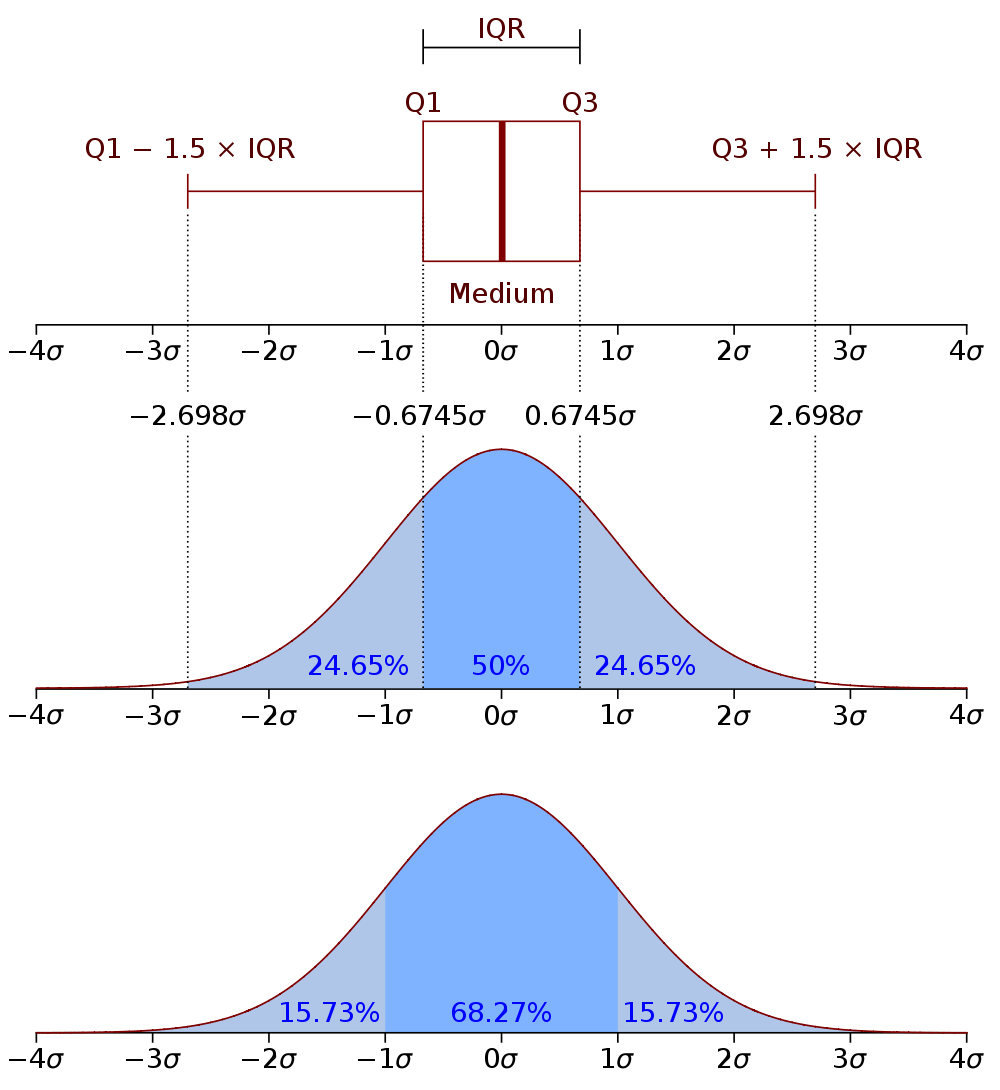
\includegraphics[width=12cm]{boxplot.png}
\caption[How to read a boxplot graph]{How to read a boxplot graph \cite{stk_boxplot}}
\label{boxlot}
\end{figure}

\chapter{SQL scripts}
\section{River assignment}
\label{app:sql_assign_river}

\lstinputlisting[language=SQL, caption={SQL source code for the river assignment process}]{./data/sql_assign_rivers.txt}


\section{Gauge assignment - modeled runoff}
\label{app:sql_assign_watergap}

\lstinputlisting[language=SQL, caption={SQL source code for the runoff assignment process - modeled runoff}]{./data/sql_assign_wg.txt}


\section{Gauge assignment - measured runoff}
\label{app:sql_assign_gauge}

\lstinputlisting[language=SQL, caption={SQL source code for the runoff assignment process - measured runoff}]{./data/sql_assign_gauge.txt}

\chapter{Python scripts}
\section{Method get{\_}dV{\_}rest()}
\label{app:get_dV_rest}

\lstinputlisting[language=python, caption={Python source code for the get{\_}dV{\_}rest method}]{./data/python_get_dV_rest.txt}

\section{Method get{\_}dV{\_}n()}
\label{app:get_dV_n}

\lstinputlisting[language=python, caption={Python source code for the get{\_}dV{\_}n method}]{./data/python_get_dV_n.txt}

\chapter{Standard data used in the model}

\section{Table containing the vertices of the turbines characteristic diagrams}
\label{app:csv_vertices}
\begin{table}
\footnotesize
 \caption{Vertices of the turbines characteristic diagrams}
 \centering
 \begin{tabular}{|c|c|c|c|c|c|}
 \hline
  Kaplan{\_}dV{\_}n&Kaplan{\_}h{\_}n&Francis{\_}dV{\_}n&Francis{\_}h{\_}n&Pelton{\_}dV{\_}n&Pelton{\_}h{\_}n\\
  \hline
  1&2&0.8&10&0.5&120\\
  100&2&80&10&30&300\\
  1000&20&1000&50&50&1000\\
  50&80&1000&100&5&2000\\
  10&80&80&800&0.5&2000\\
  1&20&5&800&&\\
  &&0.8&200&&\\
  \hline
 \end{tabular}
\end{table}
